\chapter{Usage Guide}

\label{chap:usage_guide}



\section{Multi-procedures}

\subsection{Add a new sensor}
\vspace{0.5cm}
\hfill
\hrule
\begin{lyxlist}{PC1}
\small{
\item [\textbf{Procedure:}] Add a new sensor
\item [\textbf{Scope:}] Request Management System(\emph{RMS})
\item [\textbf{Primary Actor}:] Technician
\item [\textbf{Secondary Actor(s)}:] Manager,\\
 Error Management System
\item [\textbf{Goal:}] The intention that the Technician can request a new
sensor.
\item [\textbf{Level}:] User-goal level
\item [\textbf{Main~Success~Scenario}]:\\
1. \emph{Technician} complets the diffrent input textfields and instructs the
\emph{RMS} to push a request for a sensor by pressing Push to the manager Button.
\begin{figure}[h]
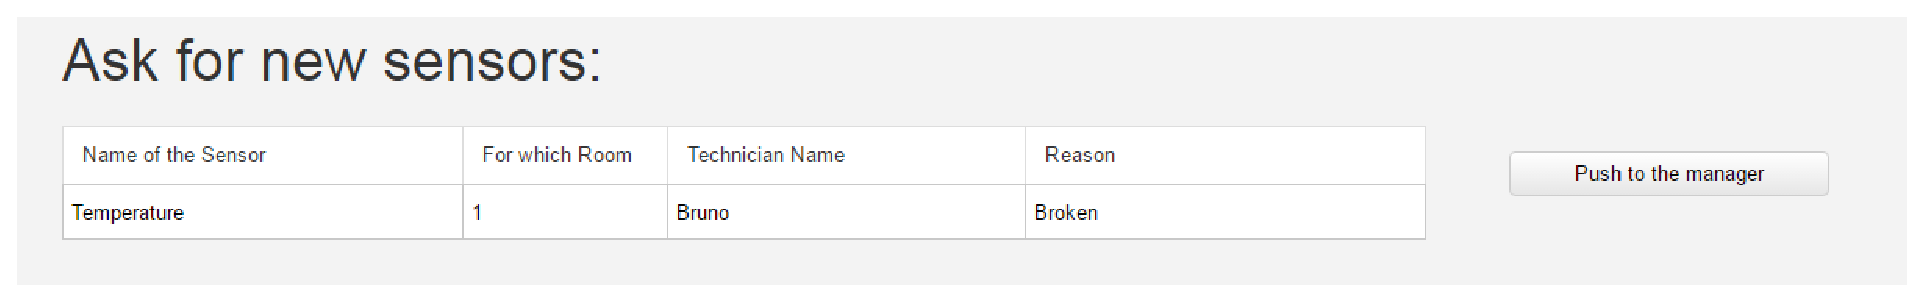
\includegraphics[width=1\textwidth]{images/AskForNewSensor.eps}
\end{figure} \\
2.\emph{RMS} displays a popup with the information entered by the Technician.\\
 \begin{figure}[h]
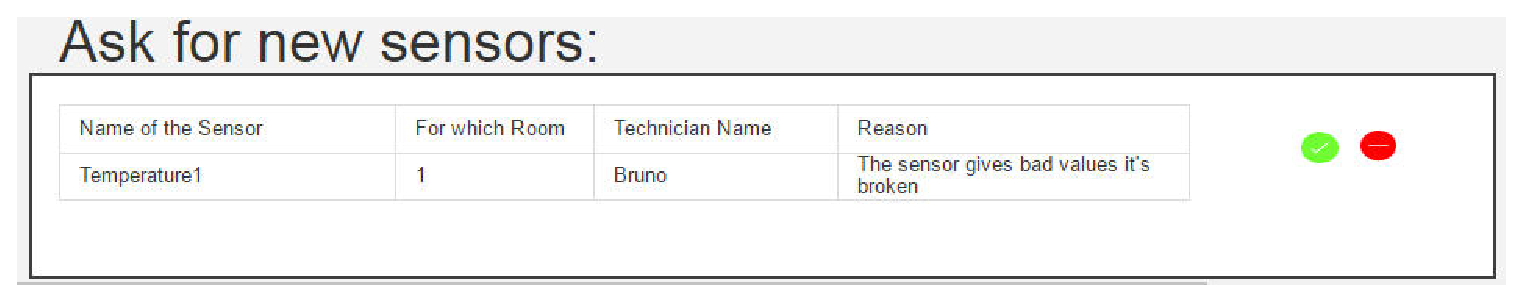
\includegraphics[width=1\textwidth]{images/AskForANewSensorPopUp.eps}
\end{figure}\\

3.\emph{Technician} accepts the information.\\

4.\emph{RMS} displays a message of validation and selects the values entered
from the \emph{Technician} and pushes them to the Manager request table.\\

5. \emph{Manager} accepts the request and instructs the \emph{RMS} to send a
confirmation to the Technician.\\

6. \emph{RMS} sets the value on the request sensor table from pending to true.\\
 \begin{figure}[h]
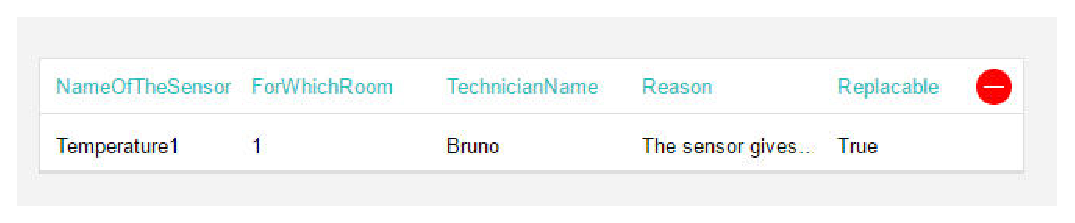
\includegraphics[width=1\textwidth]{images/AskForANewSensorTrue.eps}
\end{figure}\\

7. \emph{Technician} complets the fromular and presses add.\\
 \begin{figure}[h]
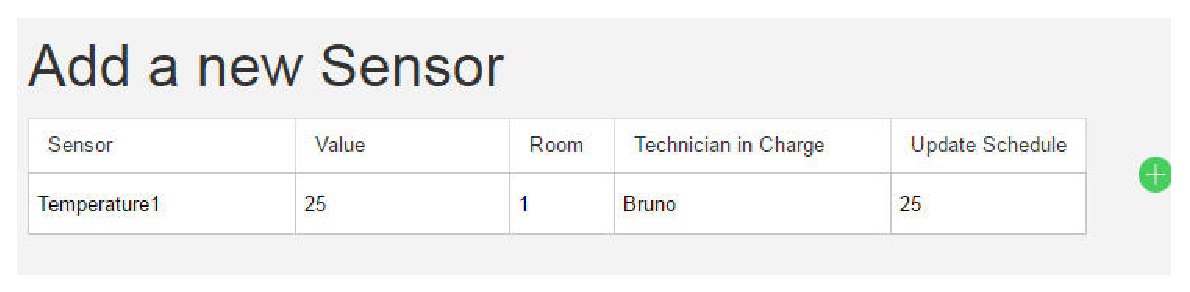
\includegraphics[width=1\textwidth]{images/AddANewSensorTechnician.eps}
\end{figure}\\

8. \emph{RMS} adds the sensor to the sensor table.\\

9.\emph{Technician} removes the sensor from the request sensor table by
pressing the red button.\\

 \begin{figure}[h]
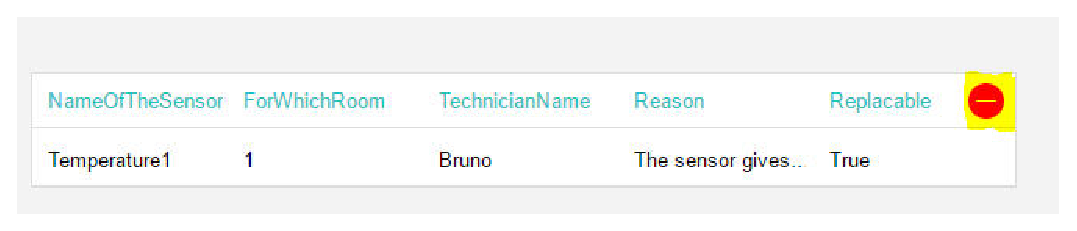
\includegraphics[width=1\textwidth]{images/RemoveSensorFromSensorRequestListTechnician.eps}
\end{figure}

10.\emph{RMS} displays a message of succesfully removed the sensor.\\
\item [\textbf{Extensions}]:\\
2.a Technician enters wrong input\\
\hspace*{0.5cm} 2.a.1 (5)-(8)\emph{EMS} displays the message error (5)-(8).
Action canceled.\\
\hspace*{0.5cm} \textbf{procedure restarts at step 1}\\
2.b Technician cancels action in the pop up.\\
\hspace*{0.5cm} \textbf{procedure restarts at step 1}\\
2.c Manager declines request\\
\hspace*{0.5cm} 2.b.1 \emph{RMS} informs \emph{Technician} that the request
has been declined.\\
}
\end{lyxlist}
\hrule
\vspace{0.5cm}

\break


\subsection{Request a different seed}
\vspace{0.5cm}
\hrule
\hfill
\begin{lyxlist}{PC1}
\small{
\item [\textbf{Procedure:}] Request a diffrent seed
\item [\textbf{Scope:}] Request Management System(\emph{RMS})
\item [\textbf{Primary Actor}:] Gardener
\item [\textbf{Secondary Actor(s)}:] Manager,\\
Error Management System
\item [\textbf{Goal:}] The intention that the Gardener can request a new
non already existing seed.
\item [\textbf{Level}:] User-goal level
\item [\textbf{Main~Success~Scenario}]:\\
1. \emph{Gardener} complets the input text fields and presses the ask new seed
button.\\
\item 
\begin{figure}[H]
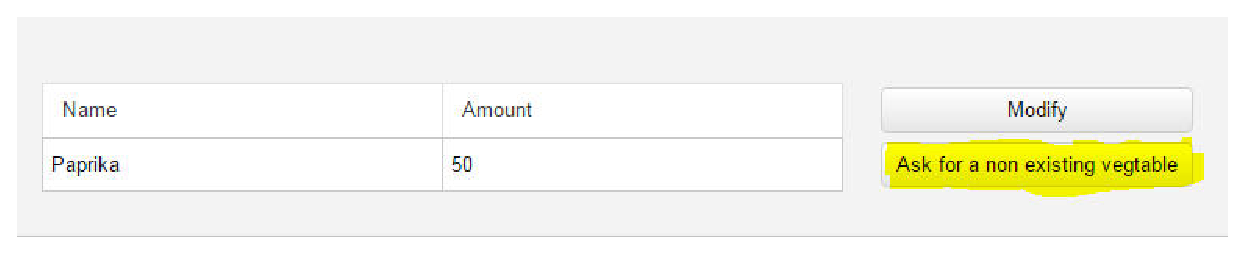
\includegraphics[width=1\textwidth]{images/AskForANonExistingVegtable.eps}
\end{figure}
2. \emph{RMS} displays a pop to show the input to the \emph{Gardener}\\
 \begin{figure}[H]
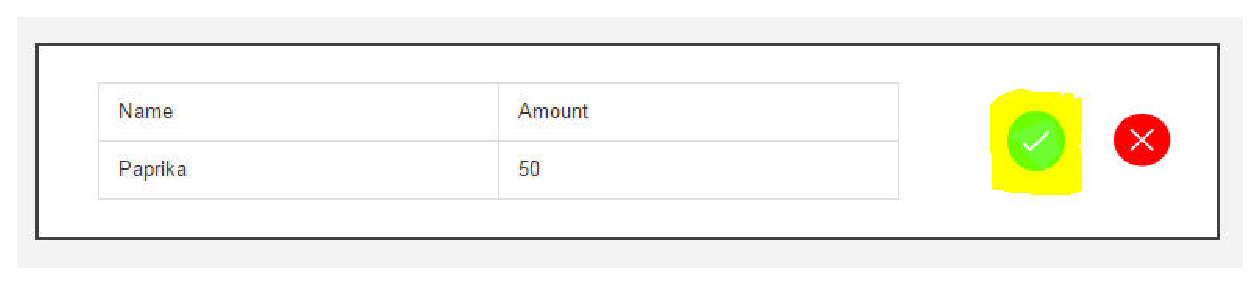
\includegraphics[width=1\textwidth]{images/AskForANonExistingVegtablePopUp.eps}
\end{figure}

3.\emph{Gardener} accepts the intput and instructs the \emph{RMS} to send
request.\\
4.\emph{RMS} pushes the input values to the manager request seed table.\\
5.\emph{Manager} accepts the request and instructs the \emph{RMS} to go on
the manager home screen.
 \begin{figure}[H]
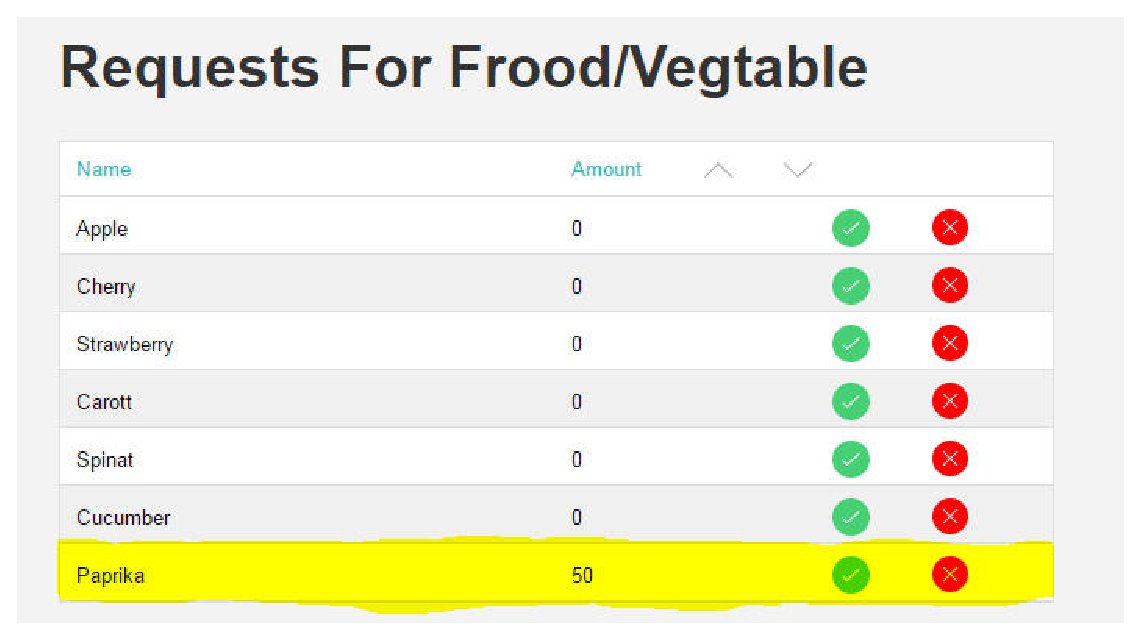
\includegraphics[width=1\textwidth]{images/AcceptRequestedCropManager.eps}
\end{figure}

6. \emph{Manager} complets the formula adding item to inventory and presses
add.\\
 \begin{figure}[H]
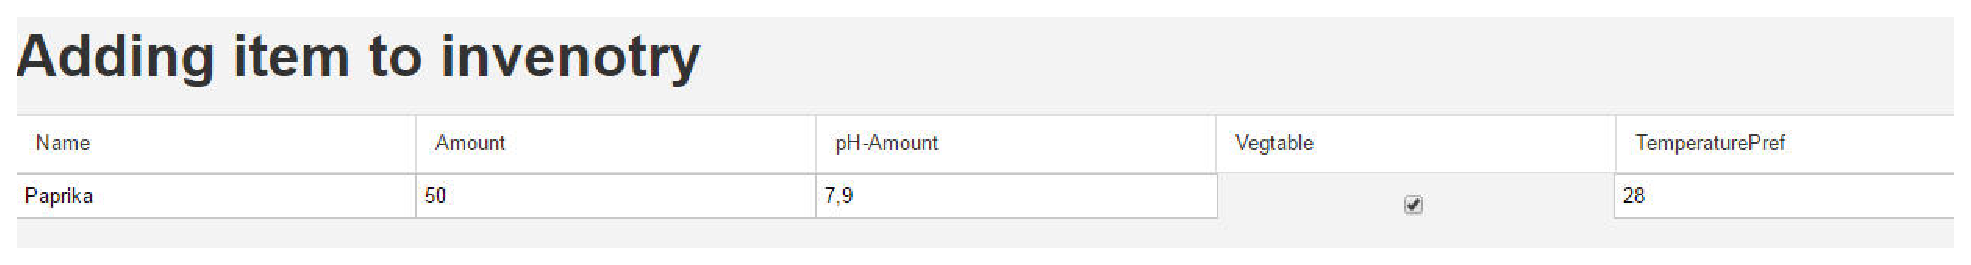
\includegraphics[width=1\textwidth]{images/AddingSeedToTheInventoryManager.eps}
\end{figure}

7. \emph{RMS} displays a pop up with the information written by the Manager.\\
8.\emph{Manager} validates the input and instructs the \emph{RMS} to update the
inventory.\\
 \begin{figure}[H]
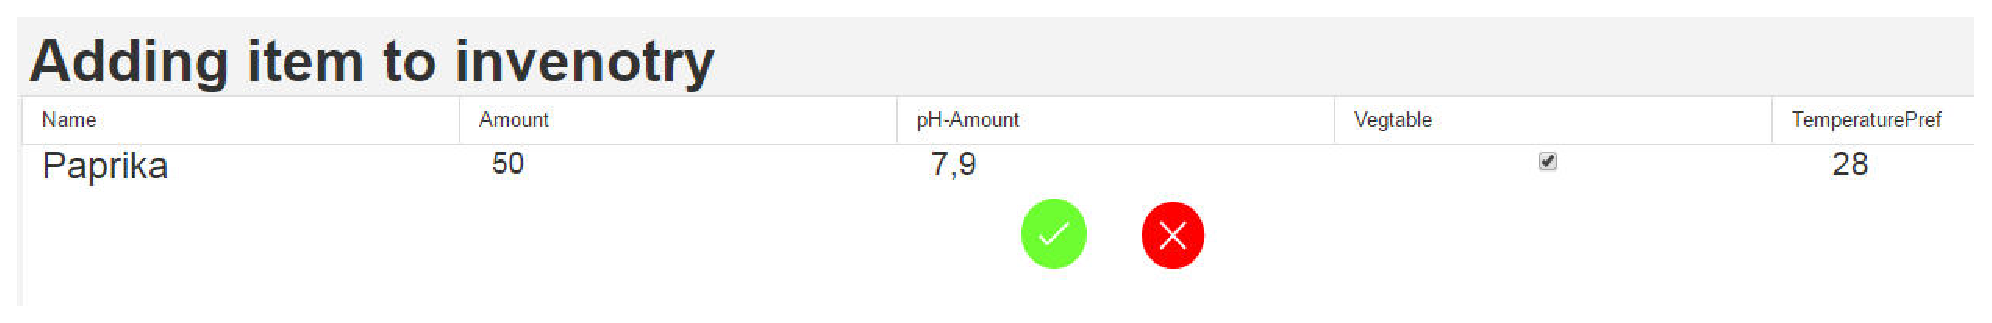
\includegraphics[width=1\textwidth]{images/AddingSeedToTheInventoryPopUp.eps}
\end{figure}

9. \emph{RMS} adds the given information to the crop invenotry table and
updates all the inventory tables.\\

\item [\textbf{Extensions}]:\\
2.a Gardener cancels the request\\
\hspace*{0.5cm} 2.a.1 {EMS} removes the pop up. Action canceled.\\
\hspace*{0.5cm} \textbf{procedure has stopped or can be resrarted at 1}
2.b Manager cancels the validation
\hspace*{0.5cm}2.b.1 {EMS} removes the pop up and cancels the action.\\
\hspace*{0.5cm}\textbf{procedure has stopped and can be restarted at 7.}
}
\end{lyxlist}
\hrule
\vspace{0.5cm}


\break
 
 
 
 

\subsection{Sign In}
\vspace{0.5cm}
\hrule
\hfill \break
\begin{lyxlist}{PC1}
\small{
\item [\textbf{Procedure:}] SignIn
\item [\textbf{Scope:}] Identified usage of the software
\item [\textbf{Primary Actor}:] User
\item [\textbf{Secondary Actor(s)}:] Greenhouse Software GS
\item [\textbf{Goal:}] Show the user GUI to manage the garden
\item [\textbf{Level}:] User-goal level
\item [\textbf{Main~Success~Scenario}]:\\
1. \emph{User} enters a username and password combination and signs in\\
2. \emph{GS} looks up the user rights defined by the administrator\\
3. \emph{GS} now show the correct Graphical User Interface (GUI) \emph{(Gardener, Technician, Manager or Administrator)} able to control the garden.
\item [\textbf{Extensions}]:\\
1.a Wrong username and password combination\\
\hspace*{0.5cm} 1.a.1 \emph{GS} notifies the \emph{User} that the entered information are wrong\\
\hspace*{0.5cm} \textbf{procedure recontinues at step 1}
}
\end{lyxlist}
\hrule
\vspace{0.5cm}


\break



\section{Mono-procedures}



\subsection{Technician}







\subsection{Manager}
\break




\subsection{Gardener}
\subsubsection{Retrive/Modify Crops from Table}

\vspace{0.5cm}
\hrule
\hfill \break
\begin{lyxlist}{PC1}
\small{
\item [\textbf{Procedure:}] Retrives vegtable or
frood the amount left of crops
\item [\textbf{Scope:}] Modify Management System \emph{MMS}
\item [\textbf{Primary Actor}:] Gardener,\\
Error Management System (EMS)
\item [\textbf{Goal:}] The intention that the gardner can retrive crops from
the inventory.
\item [\textbf{Level}:] User-goal level
\item [\textbf{Main~Success~Scenario}]:\\
1. \emph{Gardner} Complets the diffrent input text fields with there given
information and instructs the \emph{MMS} to retrive the crops by
pressing \emph{Modify}.\\

\begin{figure}
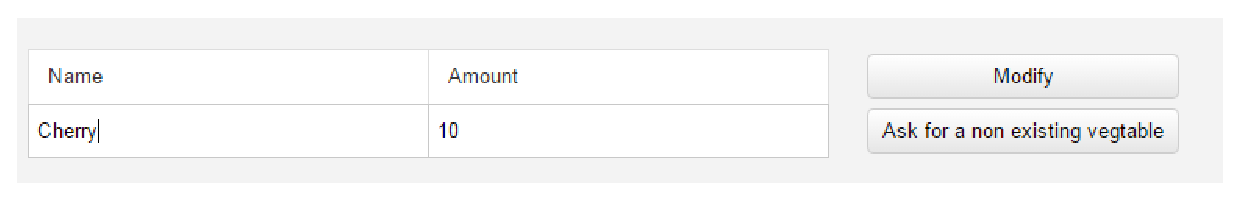
\includegraphics[width=1\textwidth]{images/RetriveCropsBase.eps}
\end{figure}

 2.{EMS} displays a pop up with the input entered by the \emph{Gardener}.\\
\begin{figure}
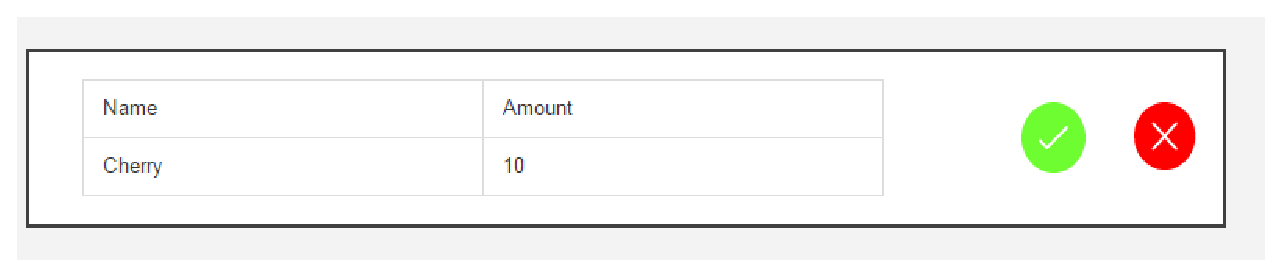
\includegraphics[width=1\textwidth]{images/PopUpRetrive.eps}
\end{figure}
3.\emph{Gardner} validates the input.\\
4.\emph{MMS} removes the crops from the table and updates the table.\\
5.\emph{MMS} enters new values to the Manager table at which time the crops
have been taken away.\\
\item [\textbf{Extensions}]:\\
2.a  \emph{Gardener} declines the pop up request to retrive crops.\\
\hspace*{0.5cm} 2.a.1 \emph{EMS}  disables the pop up and action has been
canceld\\
\hspace*{0.5cm} \textbf{procedure continues at step 1 or can be anulated}
\item 
}
\end{lyxlist}
\hrule
\vspace{0.5cm}


\break
\subsubsection{MyProcedure2MyActor2}
\ldots














